% !TEX root = ../main.tex
\chapter{Data Analysis}


\section{National Electricity Market}
Data from the National Electricity Market was studied to identify trends and features that could be used in the forecaster model. 

\subsection{Data Structure}
NEM data was collated for the period from January 2015 to December 2024 for the NSW NEM region. It contains settlement date-time, total demand for the NEM region, and wholesale price per MWh as determined by AEMO. The settlement periods are in 30 minute intervals until the 1st of October 2021, followed by 5 minute settlement periods for the rest of the data.

\subsection{Demand}
Figure~\ref{fig:nsw_demand} shows the demand in the NSW NEM over the 10 years with a 30 day rolling average. Figure~\ref{fig:acf_demand_48hr} shows the daily trends of demand whilst Figure~\ref{fig:acf_demand_365d} shows the seasonal variation in demand.

\begin{figure}[H]
    \centering
    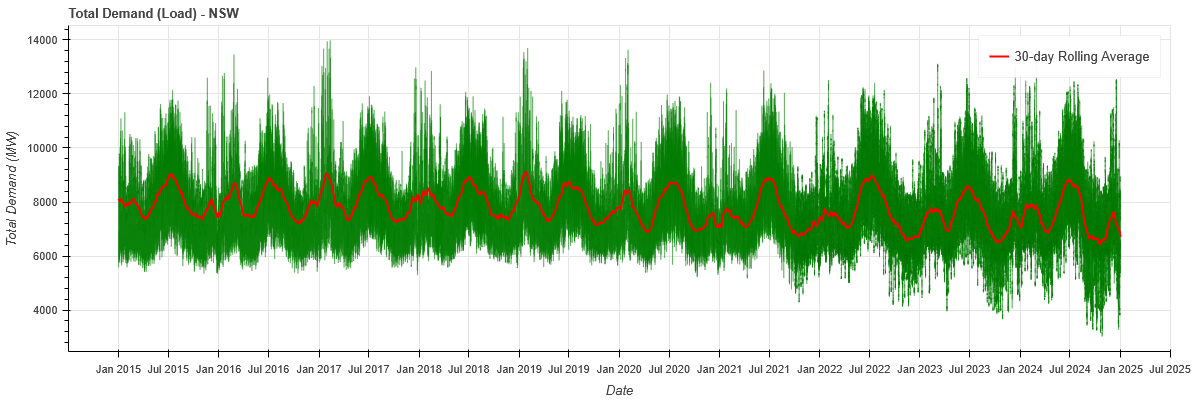
\includegraphics[width=1\textwidth]{images/NSW Demand.png}
    \caption{Demand in NSW NEM with 30 day rolling average}
    \label{fig:nsw_demand}
\end{figure}

\begin{figure}[H]
    \centering
    \begin{subfigure}[b]{\textwidth}
        \centering
        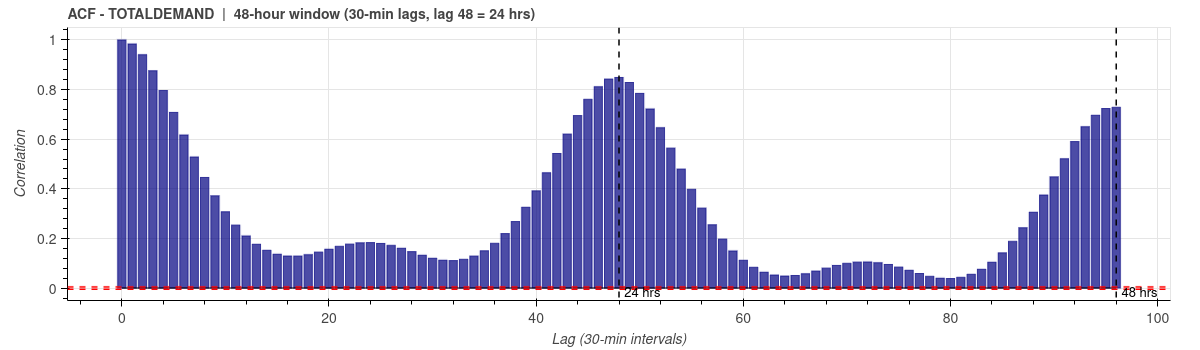
\includegraphics[width=\textwidth]{images/acf_demand.png}
        \caption{ACF - 48 Hours}
        \label{fig:acf_demand_48hr}
    \end{subfigure}
    \\
    \begin{subfigure}[b]{\textwidth}
        \centering
        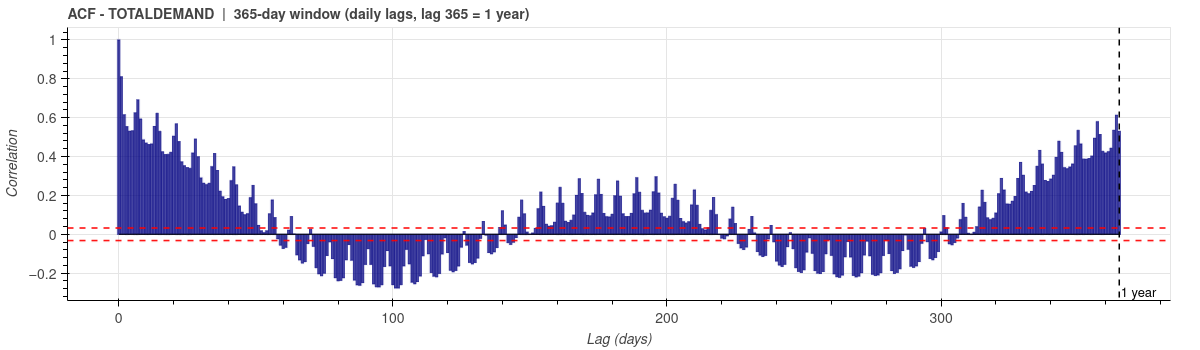
\includegraphics[width=\textwidth]{images/acf_demand_seasonal.png}
        \caption{ACF - 365 Days}
        \label{fig:acf_demand_365d}
    \end{subfigure}
    \caption{Autocorrelation analysis of demand in NSW NEM}
    \label{fig:acf_demand}
\end{figure}

\subsection{Regional Reference Price}
The data analysis on the regional reference price (RRP) found a less pronounced autocorrelation than on demand. Figure~\ref{fig:nsw_rrp} shows the wholesale price in the NSW NEM with a rolling average. The figure shows an increasing number of price spike events occurring. Figure~\ref{fig:nsw_rrp_normalised} has been normalised to remove the 1st and 99th percentiles. The results do not show the same seasonality as demand. Figure~\ref{fig:acf_pacf_rrp} however indicates that whilst long-term trends are difficult to interpret in price data, there is a strong daily trend shown by the peaks at 24 and 48 hours.

\begin{figure}[H]
    \centering
    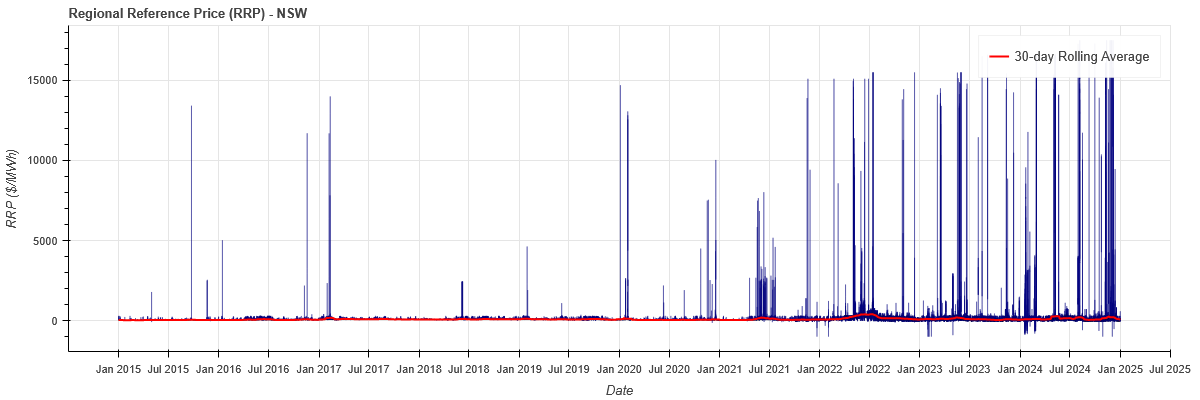
\includegraphics[width=1\textwidth]{images/NSW RRP.png}
    \caption{Wholesale price in NSW NEM with 30 day rolling average}
    \label{fig:nsw_rrp}
\end{figure}



\begin{figure}[H]
    \centering
    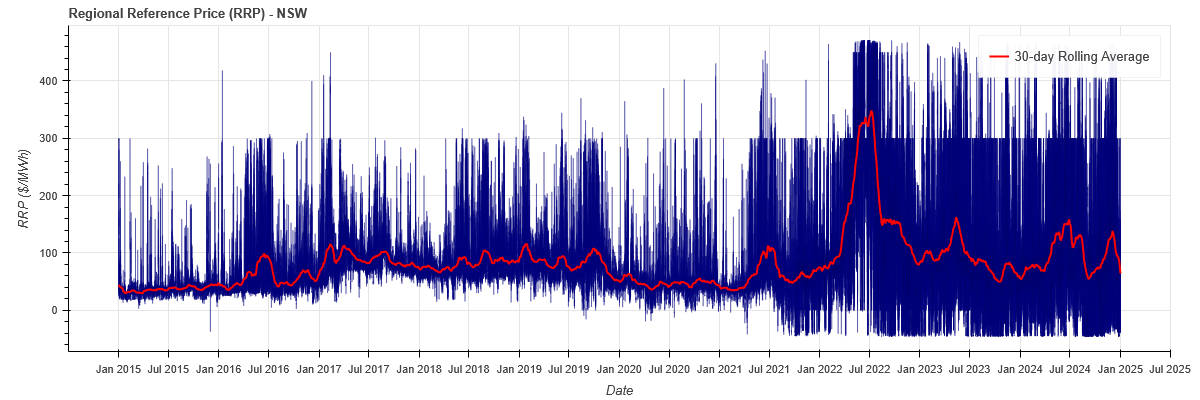
\includegraphics[width=1\textwidth]{images/NSW RRP normalised.png}
    \caption{Wholesale price in NSW NEM with 1st and 99th percentile removed}
    \label{fig:nsw_rrp_normalised}
\end{figure}

\begin{figure}[H]
    \centering
    \begin{subfigure}[b]{\textwidth}
        \centering
        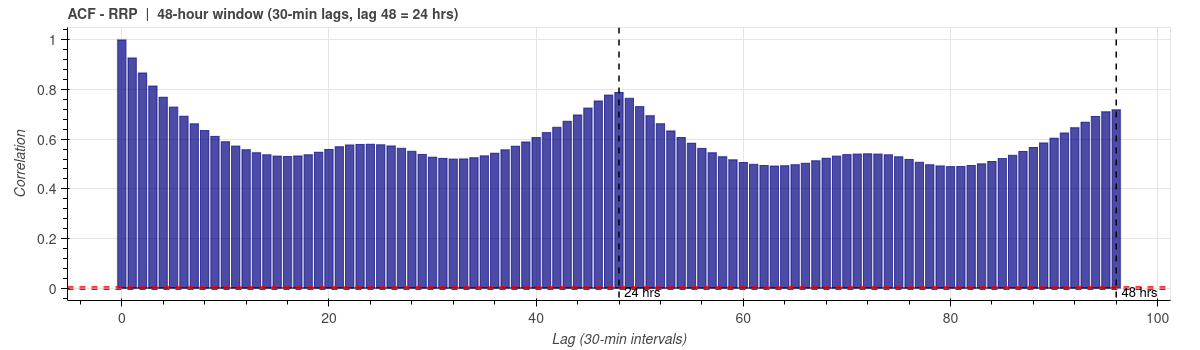
\includegraphics[width=\textwidth]{images/acf_rrp.png}
        \caption{ACF}
        \label{fig:acf_rrp}
    \end{subfigure}
    \\
    \begin{subfigure}[b]{\textwidth}
        \centering
        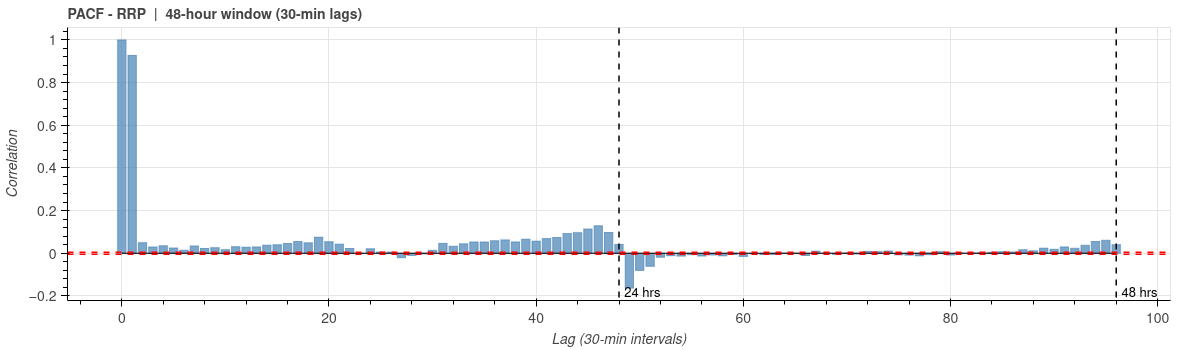
\includegraphics[width=\textwidth]{images/pacf_rrp.png}
        \caption{PACF}
        \label{fig:pacf_rrp}
    \end{subfigure}
    \caption{Autocorrelation analysis of normalised NSW NEM price series}
    \label{fig:acf_pacf_rrp}
\end{figure}


\section{Net Local Power}